\chapter{Glacio-hydrological modelling of glacierized mountain catchments}
\label{chap:discussion}

\begin{flushright}
\begin{small}
\textit{Water is the driver of nature.}\\
Leonardo da Vinci
\end{small}
\end{flushright}

\section*{Preface}

This second part of the manuscript is driven by the BERGER project, in which my PhD project is integrated, combining the glacio-hydrological modelling efforts presented here with an ecological study on the impacts of glacier retreat on aquatic communities and their adaptation in the French Alps. An unexpected shift in the initial objectives of this PhD project resulted in a lengthy investigation of machine learning methods applied to glacier evolution modelling, which impacted the initial plans for glacio-hydrological modelling. Efforts for this part of the PhD work have been focused on the technical implementation and validation of a novel glacier component for a hydrological model: J2K \citep{krause_quantifying_2002}. With this implementation, we are providing a proof-of-concept of hydrological modelling with dynamic glacier surfaces in J2K over a well-documented, high-altitude alpine catchment, and the technical means for an application on glacio-hydrological studies at a regional scale in the French Alps. This work has been done with the help of Sven Kralisch from the University of Jena (Germany). His expertise on the hydrological model used in this study has greatly helped to accelerate the development of the updated glacier module in the last months of this project. 

\section{Introduction}

Glaciers supply water that supports ecosystems and human communities both nearby and far away from glaciers \citep{ipcc_climate_2018}. The strong climatic diversity of glacierized alpine catchments enables the storage of precipitation in the form of snow and ice at high altitudes. In the European Alps, this water storage is progressively released throughout the year during the warmest months, providing a base-flow that cannot be encountered in non-glacierized catchments. At the beginning of the melt season, snow provides important water resources downstream. Once most of the snow has melted, leaving bare glacier ice exposed, glaciers continue providing freshwater resources, ensuring an uninterrupted runoff throughout the melt season \citep{huss_toward_2017}. In one of the few existing glacio-hydrological studies in the French Alps, \citet{lafaysse_influence_2011} estimated that melt water from glaciers contributed to 20\% of the August discharge of the Durance at Serre Ponçon catchment (3500 km$^{2}$). According to \citet{huss_present_2011} in a study using a simple routing of glacier discharge, glaciers contributed to 25\% of the summer low flow of the Rhone river (about 100000 km$^{2}$ in catchment size), with an even enhanced contribution during the 2003 drought. This role of glaciers as late summer buffers is currently being challenged by anthropogenic climate change. Glacier retreat in the European Alps is progressively transforming the hydrological regime of high-mountain catchments, with potential environmental and social impacts \citep{zekollari_modelling_2019}. In the French Alps, the local population have a strong dependency on water resources, using them for agriculture, hydropower generation and domestic use. The regional socioeconomic model of many alpine valleys is built around mountain tourism, with a strong dependency on the cryosphere, both as a tourism attraction \citep{schut_sport_2013, spandre_winter_2019} and as an electricity generation source \citep{schaefli_role_2019}. Moreover, late summer runoff from glaciers provides reliable water resources for domestic use, industries and agriculture. The decrease in glacier freshwater contributions has ecological impacts as well, affecting biodiversity in glacier-fed rivers \citep{cauvy-fraunie_global_2019} and in humid areas that no longer receive runoff during the warmest period of the year \citep{carlson_monitoring_2020}. Glaciers provide cold water resources that help regulate the temperature, flow regimes, sediment concentration and nutrient supply of mountain streams \citep{huss_toward_2017}. These cold waters are essential to some specialized species, whose survival will be challenged by glacier retreat \citep{lencioni_glacial_2018, cauvy-fraunie_global_2019}. Alternatively, these changing streams can be quickly colonized by aquatic communities adapted to higher water temperatures, increasing competition between species  \citep{robinson_ecosystem_2014}. Anticipating these future hydrological changes is of paramount importance in order to correctly adapt and manage future water social and environmental needs. 

Hydrological models can provide answers to these questions, predicting the hydrological evolution under different future climate scenarios. In France, multiple hydrological models are being developed and used for research and operational purposes. At one end of the spectrum of model complexity, the lumped GR rainfall-runoff models, with the CemaNeige snow component \citep{coron_suite_2017}, use a simplified modelling approach with catchment-scale representations of the transformation of precipitation into discharge. They rely on the calibration of 1 to 6 parameters (depending on the model variant and time-step), and do not include a glacier component. This limits their usability in high-altitude, upstream catchments where observational data for calibration is scarce and glaciers may play an important role.  At the other end of the complexity spectrum, the physics-based SIM (SAFRAN-ISBA-MODCOU) model combines a meteorological analysis system (SAFRAN), with a land surface model (ISBA) and a hydrogeological model (MODCOU) developed by the Mines de Paris \citep{habets_safran-isba-modcou_2008}. For research purposes, it has been adapted to alpine areas by incorporating elevation bands, aspect classes, and glacier melt and retention of underground water \citep{lafaysse_influence_2011}. However its adaptation and deployment over the entire French alpine region, including glacierized areas, is highly demanding \citep[e.g.][]{lecourt_physically-based_2018} and has not been considered yet. For more operational applications, the reservoir-based MORDOR model \citep{paquet_evolution_2004}, developed by Électricité de France (EDF), has a more intermediate complexity. It is actively  used to forecast runoff in mountain catchments in France and to anticipate changes in hydropower production, both for short and long term periods. However this model is not open to applications outside the scope of EDF operational and research objectives. Finally, The GSM-Socont model \citep{schaefli_conceptual_2005}, a Swiss semi-distributed glacio-hydrological model, has been recently applied to perform projections of the Arve watershed in the Mont-Blanc massif through the 21${st}$ century \citep{laurent_impact_2020}. Out of all these models, only the GSM-Socont model includes a dynamic representation of glaciers, and \citet{laurent_impact_2020} is the first study of this kind in a French glacierized catchment. The vast majority of hydrological models deployed in France have none, or a very simplified representation of glaciers, including them as static ice reservoirs. Some models do have such glacier modules, but they are not activated due to a lack of data to calibrate and validate them. Such a representation is problematic in the current context of glacier retreat, neglecting future changes in hydrological regimes driven by glaciers. 

This static representation of glaciers is also found in the J2K hydrological model \citep{krause_quantifying_2002}, developed at the University of Jena (Germany). J2K is a distributed open-source model, based on Hydrological Response Units (HRUs), homogeneous spatial units in terms of hydrological processes. It allows the representation of multiple physical processes, land use covers, pedology, geology and topography. Moreover, the representation of multiple anthropogenic water uses, such as agriculture irrigation or reservoir management dams can be taken into account in the model. J2K is being used by a large community of hydrologists, both in France and internationally, for a wide variety of geographical configurations \citep{krause_quantifying_2002, nepal_understanding_2014, braud_j2000-rhone_2017}. J2K has already been applied to glacierized catchments in the Himalayas \citep{nepal_understanding_2014}, but simulations have only been performed for past periods, keeping the glacier surface area constant in time. In this chapter, I present an updated glacier module for J2K, including a dynamic representation of glaciers. We introduce and validate this new implementation in a partially-glacierized (4.5 \%) alpine catchment in the French Alps: the Arvan catchment in the Grandes Rousses massif. By introducing glacier evolution in a distributed hydrological model, we aim at improving hydrological simulations and discharge projections out of glacierized catchments, in support of diverse applications but primarily to assess the impacts of changes in glacier discharge on aquatic communities living in glacier-fed streams. Such an application requires a distributed hydrological model able to provide discharge information on upstream sub-catchments. 

\section{Methods}

\subsection{Study area}

The Arvan catchment (58.8 km$^{2}$, Fig. \ref{hydro:fig1}) is a partially glacierized alpine catchment, located in the Grandes Rousses massif, between 1368 and 3373 m a.s.l. It includes the Saint-Sorlin Glacier (2.069 km$^{2}$ in 2015, 3.5\% of glacial coverage at catchment scale), being the glacier with the second longest mass balance observation series in France (1957-present). Two villages are located within the catchment: Saint-Sorlin-d'Arves and Saint-Jean-d'Arves, with the latter including water flow measurements for the 2000-2016 period. This study site has been chosen due to its wealth of glaciological, meteorological and hydro-biological data, providing an adequate testbed to validate the modelling approach within the context of the BERGER project.

\begin{figure}[h]
\centering
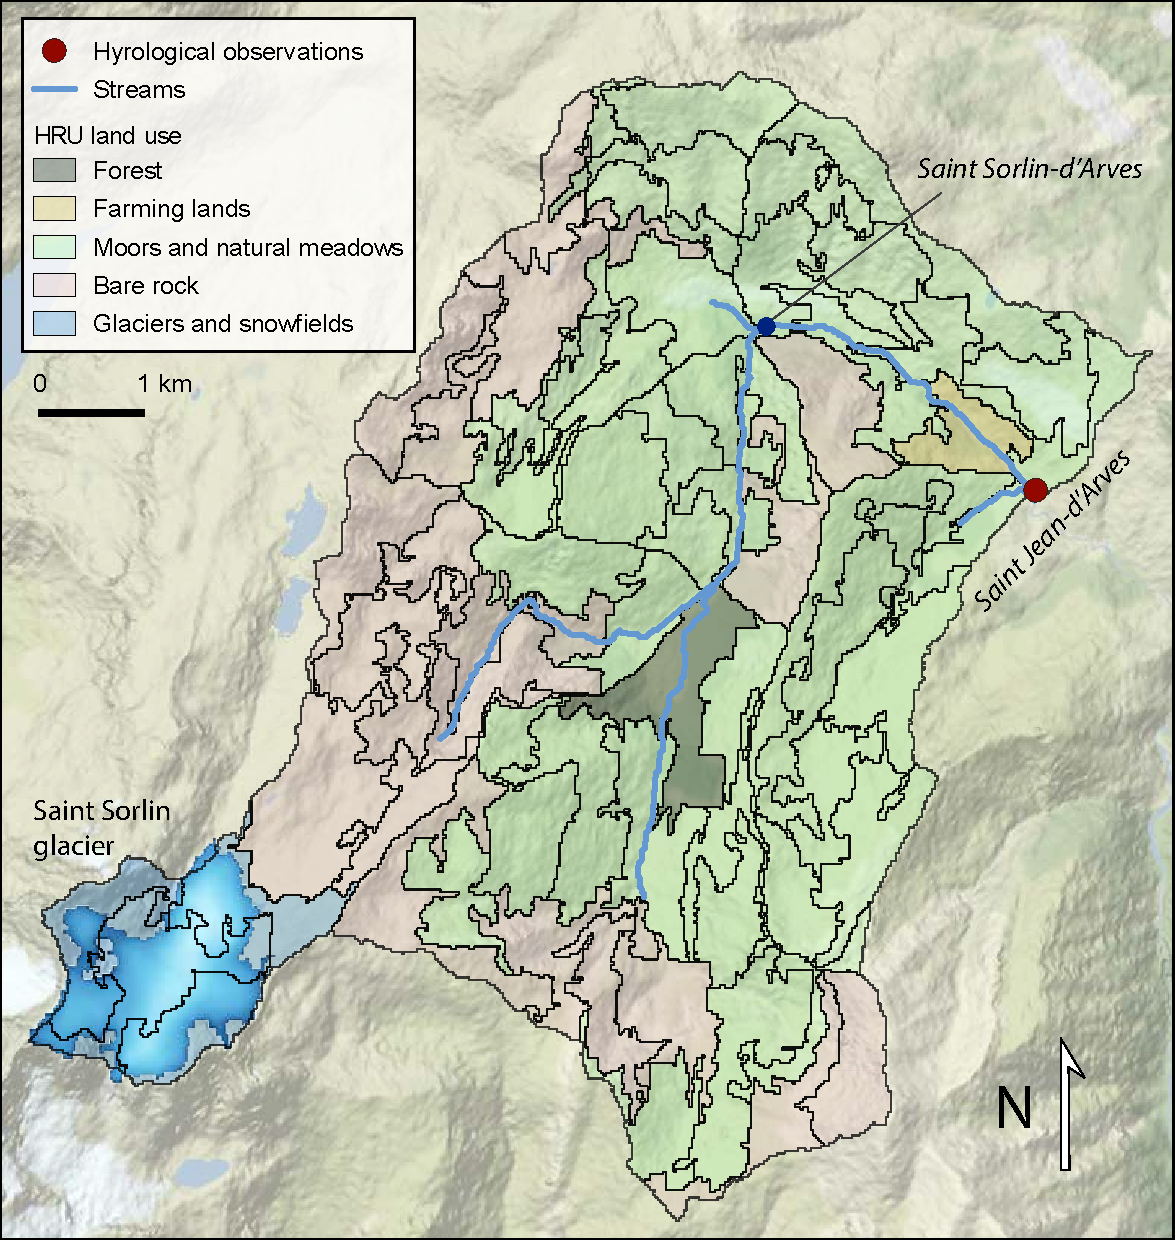
\includegraphics[width=12cm]{Figures/hydro/Figure_2.pdf}
\caption{The Arvan catchment at Saint-Jean d'Arves, with its division into HRUs and their main land use. } 
\label{hydro:fig1}
\end{figure}

\subsection{Data}

This work has been implemented in a version of J2K dedicated to the Rhône river catchment, situated in France and Switzerland. Therefore, most of the datasets used (except the climate data) have a full coverage of this geographical region.

\subsubsection{Climate}

The J2K hydrological model is forced with climate data coming from SPAZM \citep{gottardi_statistical_2012}. SPAZM is a statistical method to interpolate meteorological data, particularly precipitation, in mountain areas. This interpolation has been applied on French mountainous regions, based on an observational network, taking into account the local orography and the main atmospheric patterns bringing precipitation. With a resolution of 1 km$^{2}$, this dataset is well adapted to representing the complex meteorological conditions of a glacierized alpine catchment. Temperature and precipitation are available from the year 1953 until the end of the year 2012, which suit the needs of J2K.

\subsubsection{Land cover}

Land cover use is determined by the Corine Land Cover 2006 (CLC2006) European database. It has a minimum vectorial detail of 25 ha and it takes into account a maximum of 44 different land cover uses. Land use data is used to determine certain variables in different hydrological processes, such as the surface albedo or the leaf area index. 

\subsubsection{Pedology}

Pedology information is used to estimate the size of the superficial soil reservoirs in the model. The following databases have been used to describe pedology: The Soil European Database, providing soil thickness data; and the ECOCLIMAP database, with a 1 km resolution, describing soil texture. The representation of these superficial soil reservoirs is based on \citet{sauquet_risk_2014}, adapted for mountain territories. 

\subsubsection{Geology}

Geology data is taken from the Bureau des Recherches Géologiques et Minières (BRGM) dataset, grouped in eight different classes, five of which are dominant in the French Alps: fluvioglacial deposits, shale and metamorphic rocks, detrital rocks, limestone and marls. In J2K, geology is used to determine the size and time to empty the deep ground reservoirs. 

\subsubsection{Hydrology}

Hydrological observations at the Saint-Jean-d'Arves station (Fig. \ref{hydro:fig1}), are available with a daily frequency for the 2000-2016 period. This data is compiled as part of DREAL Rhône-Alpes's database of hydrological observations \citep{brigode_summary_2020}. This station measured an average interannual flow of 1.8 m$^{3}$/s, with 10\% of temporal gaps for this period and a low reliability of winter measurements. During winter, ice forms in the river, altering the measured water altitude, and in autumn strong rains can often carry large rocks which alter the measured river section. This introduces time gaps or artefacts in the observations, reducing their reliability for certain periods. 

\subsubsection{Glaciology}

Several different datasets are available for the Saint-Sorlin Glacier. Seasonal (winter and summer) point MB data from the GLACIOCLIM French national observatory are available at 30 different points since 1995. Glacier-wide MB observations, performed every year in September, cover the 1957-2019 period. Seasonal glacier-wide MB data were computed specifically for the 2000-2010 period \citep{davaze_monitoring_2018}. Glacierized surface areas for this glacier proceed from the results of model simulations using the ALPGM model, introduced in Chapter 2. 

\subsection{The J2K hydrological model}

J2K is an open-source hydrological model coded in Java. It is structured in Hydrological Response Units (HRUs), irregular spatial divisions representing homogeneous conditions from a hydrological point of view. HRUs are determined by a combination of different spatial data, such as the surface slope, altitudes from a DEM, vegetation cover, geology and the distribution of sub-catchments. For the J2K model version used in our study, HRUs are determined by taking into account the sub-catchments with control gauging stations from the hydrological network of observations. These control points are used for model calibration and validation, enabling a comparison of model simulations with observations. The automatic generation of HRUs is performed with a special tool named HRU-delin, providing the modelling structure for any given catchment with the required data. The physical characteristics of each HRU are stored in specific files, which are used by the model to simulate different hydrological processes. 

Simulations are performed in two nested loops, a first one iterating every timestep (days in most cases), and another one iterating in space (HRUs). Total precipitation can be partially intercepted by vegetation, whose remaining fraction that reaches the ground will be further divided into infiltrated and surface runoff (RD1) fractions. Infiltrated water will first fill a Large Pore Space (LPS) reservoir, which can then be transferred towards a Medium Pore Space (MPS) reservoir (Fig. \ref{hydro:fig2}). Evapotranspiration (ET) is mainly retrieved from water intercepted by vegetation and water available in the MPS reservoir. It is computed on vegetation following the Penman-Monteith reference potential evapotranspiration \citep{howell_penman-monteith_2004}. J2K allows ground water to form subsurface runoff (RD2) if the surface slope is steep enough or the substrate has low infiltration. The remaining fraction is assumed to percolate towards a deep reservoir (RG1). The simulated total water flow within an HRU is equivalent to the sum of the runoff, the subsurface flow and a slow flow from the deep reservoir. Water flow is routed among HRUs via streams if the HRU is located on a valley bed. Conversely, HRUs not containing a water stream route their water flow towards neighbouring HRUs using a simplified kinematic wave method \citep{chen_surface_1970}. Every type of water storage (e.g. RD1, RD2) from each HRU is routed separately until reaching the catchment's outlet. 

\begin{figure}[h]
\centering
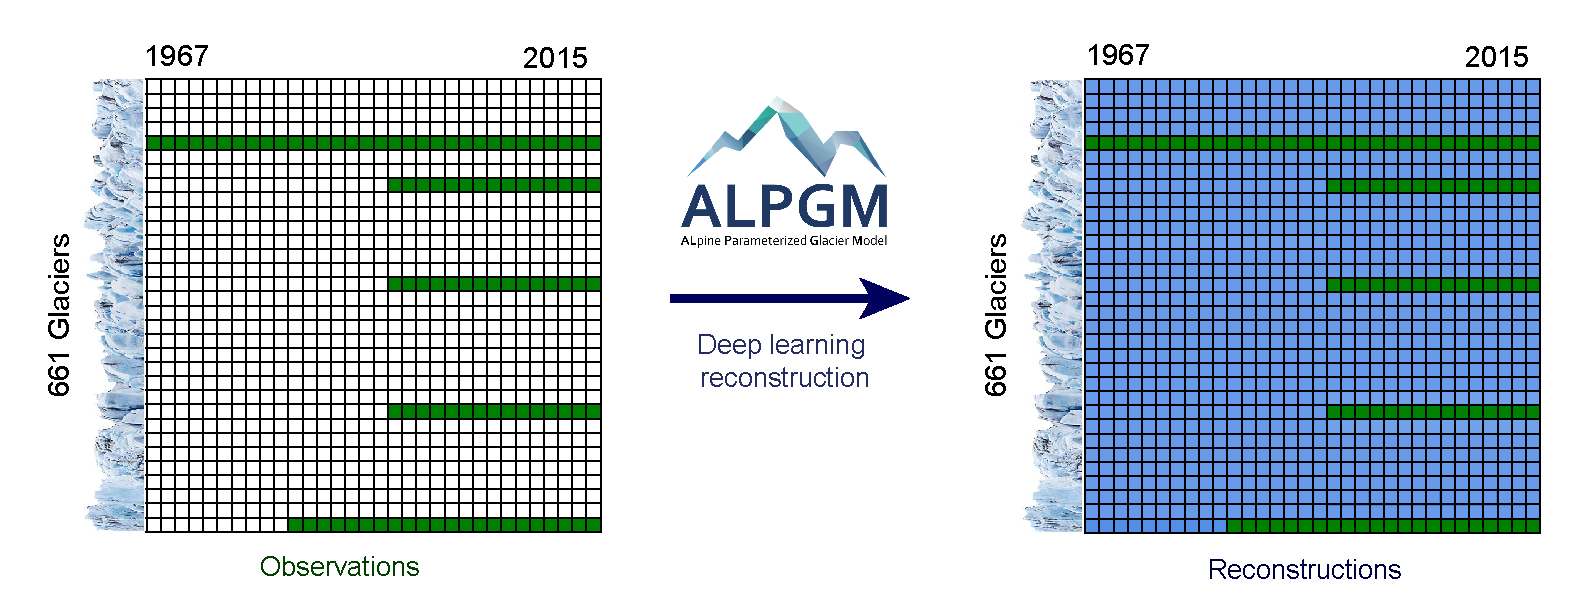
\includegraphics[width=8cm]{Figures/hydro/Figure_1.png}
\caption{Workflow of the J2K hydrological model. \textit{Taken from the J2K documentation.}} 
\label{hydro:fig2}
\end{figure}

J2K establishes a simulation workflow using temporal (HRU-Loop) and spatial (Time-Loop) contexts, which iterate and perform simulations for each HRU and day of a given catchment and time period. These contexts are implemented in the Jena Adaptable Modelling System (JAMS) platform, in which J2K is integrated. The simulation of specific hydrological processes are performed in components, being separate entities taking a given set of input parameters, processing them and returning multiple output parameters. 

\subsection{Existing glacier module}

The previously existing glacier module developed for the Himalayas is based on a snow processing component and a glacier MB component. In our case study, we used the snow processing component from the Rhône version of J2K (also used over the ice-free parts of the catchement), combined with the glacier MB component from the Himalayas version of the model.

In order to compute the glacier MB and the resulting runoff, the snowpack on the glacier is first processed with the snow component, determining the characteristics of snow on the glacier. This component simulates the accumulation and melt of the snowpack caused by air temperature or rain. The thermal characteristics of the snowpack are also taken into account by means of a cold content. Here, we show only the most relevant equations, as these processes were already available in J2K prior to this PhD work.

Accumulation and melt are computed based on the following temperature (Eq. \ref{hydro:eq:1}).

\begin{equation} \label{hydro:eq:1}
 T_{acc} = T_{melt} = \frac{T_{min} + T_{max}}{2}
\end{equation} 

If $T_{melt}$ exceeds a certain threshold value (here chosen to be 0ºC) the snowpack transitions from accumulation phase to melt. The amount of energy available for melt is computed with a daily timestep via a degree-day approach (with $\alpha_{snow}$ as daily degree-day factor), where the advected energy from the rain is also accounted for. The sum of these two components gives the potential snow melt rate ($M_{p}$, in mm), defined by equation \ref{hydro:eq:2}.

\begin{equation} \label{hydro:eq:2}
 M_{p} = \alpha_{snow} \cdot T_{melt} + r_{factor} \cdot rain \cdot T_{melt} 
\end{equation} 

In this equation $r_{factor}$ can be calculated based on heat capacity and latent heat of fusion , under the hypothesis that rain water is at air temperature prior to warming and melting the snowpack, resulting in an $r_{factor}=0.0125$ °C$^{-1}$. 

Density and snow height are diagnosed from the snow water equivalent (SWE) based on fresh snow density (taken as 300 kg/m$^{3}$) and accounting for melt and settlement processes due to rain-on-snow, according to \citet{bertle_effect_1966}. The snowpack can store liquid water in its pores up to a certain critical density. When a certain amount of liquid water is reached with respect to the total SWE (about 40-45\%), rendering the density higher than a critical value $d_{crit}=700$ kg m$^{-3}$, all liquid water in excess is immediately released. In addition, liquid water within a wet snowpack is also released as runoff at a slower pace, depending on the snowpack saturation degree. The water released from the snowpack ($q_{snow}$), in mm m$^{-2}$, is computed as the sum of these two contributions  (Eq. \ref{eq:3}).

\begin{equation} \label{hydro:eq:3}
q_{snow} = H \cdot max(d - d_{crit}, 0) + WC \cdot (1-e^{(1-(d_{crit}/d)^4)})
\end{equation} 

where $d$ is the snowpack density, $H$ the snow height and $WC$ the snowpack liquid water content. 

If no snow is present in a given glacierized HRU, ice melt can occur. This is computed using a temperature-index melt model \citep{hock_temperature_2003}, following equation \ref{hydro:eq:4}.

\begin{equation} \label{hydro:eq:4}
q_{ice} = \alpha_{ice } \cdot(T_{melt} - T_{base})
\end{equation} 

where $\alpha_{ice}$ is the melt factor specific for ice and $T_{base}$ is a user-defined temperature beyond which melt is triggered, in our case 0ºC. 

This previously existing glacier module implemented in the Himalayas also takes into account the effects of debris cover, which will not be described here since they have not been used in this work. 

Finally, rain runoff, snow melt and ice melt are further adapted taking into account a storage and release time within the snowpack and glacier, respectively. This inertia is accounted for by three calibration coefficients, $k_{rain}$, $k_{snow}$ and $k_{ice}$. Here, we relied on calibration from previous studies to infer the value of theses coefficients ($k_{rain}$=5, $k_{snow}$=5, $k_{ice}$=10). These updated runoff values are computed following equations \ref{hydro:eq:5}, \ref{hydro:eq:6} and \ref{hydro:eq:7}.

\begin{equation} \label{hydro:eq:5}
Q_{rain} = q_{rain(t-1)}\cdot (1-e^{-(1/k_{rain})}) + q_{rain(t)} \cdot e^{-(1/k_{rain})}
\end{equation} 

\begin{equation} \label{hydro:eq:6}
Q_{snow} = q_{snow(t-1)}\cdot (1-e^{-(1/k_{snow})}) + q_{snow(t)} \cdot e^{-(1/k_{snow})}
\end{equation} 

\begin{equation} \label{hydro:eq:7}
Q_{ice} = q_{ice(t-1)} \cdot (1-e^{-(1/k_{ice})}) + q_{ice(t)} \cdot e^{-(1/k_{ice})}
\end{equation} 

where $q_{rain(t-1)}$ is the rain runoff from the previous timestep, $q_{snow(t-1)}$ is the snow water release from the previous timestep, $q_{ice(t-1)}$ the ice runoff from the previous timestep.

\subsection{An updated glacier module}

We updated the already existing glacier module from the J2K model version used in the Himalayas \citep{nepal_understanding_2014}, creating a new module named \textit{GlacierModuleAlps}. Several components of J2K have been adapted in order to take into account these changes in glacier surface area. 

\subsubsection{Glacier dynamics}

A Python package named \textit{Glaciers-to-J2K} has been created, which automatically computes the glacierized fraction of each HRU based on polygons with the extension and surface type of each HRU and annual glacier boundaries. Glacier boundaries can proceed from any glacier model providing annual gridded glacier extents. \textit{Glaciers-to-J2K} computes the glacierized and non-glacierized fraction of each HRU by overlapping HRU outlines with annual glacier extents. Then, these fractions are interpolated with a daily timestep throughout a given ablation sub-period, with a default period between June 1$^{st}$ to September 30$^{th}$. This enables a daily representation of glacier area evolution, necessary for hydrological simulations with J2K. These time series are stored in a \textit{.dat} file.

In J2K, the generation of HRUs for a certain catchment can only be done prior to model simulations. The extent and content of HRUs is static in time, preventing the model from making them evolve throughout a simulation. This specificity of J2K makes it difficult for the model to include a dynamic representation of glaciers, explaining why all simulations for glacierized catchments have so far been performed with static glacierized areas \citep{gao_test_2012, nepal_understanding_2014}. In order to overcome this limitation, we have developed an approach allowing the introduction of glacier evolution through time, based on prescribed glacier surface areas fed to the model at a regular timestep (e.g. daily in this study). 

Two new components named \textit{GlacierFractionReader} and \textit{GlacierFractionAssigner} have been added, responsible for reading the daily glacierized fractions for each HRU and assigning them to the right HRU during the temporal (Time-Loop) and spatial (HRU-Loop) iterations. 

\subsubsection{Glacier mass balance and runoff}

Within the HRU loop of the model, if the glacierized fraction of a given HRU is different than zero, a glacier is detected and the simulation of glacier runoff is triggered. The snow and ice runoff are computed following the equations \ref{hydro:eq:5}, \ref{hydro:eq:6} and \ref{hydro:eq:7}. The resulting daily glacier MB for each HRU is calculated from the input liquid and solid precipitation and the output ice ($Q_{ice}$), snow ($Q_{snow}$) and rain ($Q_{rain}$) runoff (Eq. \ref{hydro:eq:7}).

\begin{equation} \label{hydro:eq:7}
MB = (rain + snow - Q_{ice} - Q_{snow} - Q_{rain}) 
\end{equation} 

The main novelty from this updated module is the fact that we are scaling the precipitation falling on glaciers with the prescribed glacierized fractions ($g_{fraction}$). This means that for HRUs containing a glacier, the input precipitation is split between the glacierized and non-glacierized fractions. These fractions evolve with a daily timestep, enabling the correct representation of glacier evolution through time in J2K. The glacierized area for each HRU is also updated with a daily timestep by multiplying the HRU area by the glacierized fraction.

\subsubsection{Mass balance calibration}

The updated glacier module computes glacier MB with a daily timestep using a temperature-index model \citep{hock_temperature_2003}. This type of model relies on an empirical relationship between air temperature and melt, which is clearly observed in the French Alps despite presenting a high spatial variability. Temperature is known to correlate well with melt energy, mainly through short-wave radiation \citep{sicart_glacier_2008}. In order to correctly calibrate glacier MB, three parameters can be tuned: a precipitation rate factor specific for the glacier, a snow melt factor ($\alpha_{snow}$) and an ice melt factor ($\alpha_{ice}$). Precipitation is known to be underestimated at high altitudes (> 3000 m a.s.l.) in meteorological reanalysis datasets due to the lack of in-situ observations. This has been highlighted for SAFRAN \citep{vionnet_sub-kilometer_2019} and is also likely to be the same case for the SPAZM dataset, even though it integrates more observations for high altitude areas. This means that increasing precipitation via a multiplicative correction factor is often needed in order to correctly reproduce accumulation rates on glaciers. 

In order to calibrate the snow and ice melt factors and the precipitation multiplicative corrective factor in J2K for the Saint-Sorlin Glacier (Eq. \ref{hydro:eq:3} and \ref{hydro:eq:4}), we used seasonal (winter and summer) glacier-wide MB direct observations from the GLACIOCLIM glacier observatory. The precipitation correction factor was calibrated based on winter MB data, and the ice and snow melt factors on summer MB data. Due to time constraints, this calibration was performed manually. J2K includes a parameter optimization module, but the recalculation of glacier MB from a daily to seasonal frequency was performed outside J2K, in the \textit{Glaciers-to-J2K} Python package, in order to accelerate the development. In the future, this recalculation should be moved inside J2K to enable the automatic calibration of the precipitation correction factor and melt factors for ice and snow for large catchments.

\subsubsection{Non-glacierized fraction}

Glacierized HRUs might contain a non-glacierized fraction as well. The precipitation outside the glacier, within the previously existing workflow in J2K, is multiplied by the non-glacierized HRU fraction ($1 - g_{fraction}$). This enables an accurate separation between glacierized and non-glacierized runoff contributions for each HRU. As for the glacierized HRUs, the non-glacierized area is computed daily by multiplying the HRU total area by the non-glacierized fraction.

\section{Results}

This updated glacier module for the J2K hydrological model has been implemented and validated in the Arvan glacierized catchment at Saint-Jean d'Arves in the French Alps (Fig. \ref{hydro:fig1}). In this catchment configuration, the Saint-Sorlin Glacier occupies four different HRUs, whose glacierized fraction and surface area have been computed for every year between 2003 and 2012 using glacier ice thickness data simulated with ALPGM \citep{bolibar_alpgm_2020}.

\subsection{Glacier dynamics}

The evolution of glaciers in the updated glacier module of J2K is represented with prescribed annual glacier extents taken from an independent glacier evolution model. For this case study, ALPGM provided annual glacier ice thickness data from the year 2003, where initial glacier ice thickness data are available from \citet{farinotti_consensus_2019}. The 1985-2003 period was used as a spin-up period for the model, in order to correctly initialize the water reservoirs and snow pack. During the spin-up period, since no glacier ice thickness data is available, the extent of the glacier was kept the same as the year 2003. We consider this approximation to be acceptable, taking into account that this simulated period is only used as spin-up. The match between the initial glacier ice extent and the catchment HRUs was not perfect, with small parts of the glacier exceeding the HRUs extent (Fig. \ref{hydro:fig1}). The prescribed glacier surface areas by the ALPGM glacier model also carry uncertainties, particularly from the initial glacier ice thickness \citep{bolibar_deep_2020}. Simulated glacier MB data for this period have a very small error (Fig. 3.7), and the parameterization used to update the glacier geometry was specifically calibrated for this glacier. These uncertainties resulted in the simulated glacier geometry only evolving in thickness but not extent between 2004 and 2006. This can be seen in the prescribed glacier surface area changes, which do not evolve until early 2006 (Fig. \ref{hydro:fig3}). As soon as the prescribed glacier surface area evolves, J2K captures a realistic glacier area evolution during the ablation season. Hence, the overall glacier surface area in J2K is correctly represented, despite the slight mismatches in glacier and HRU data. The Saint-Sorlin Glacier displayed a total surface area of 2.79 km$^{2}$ in the year 2003 \citep{gardent_multitemporal_2014}, close to the 2.66 km$^{2}$ obtained in J2K (Fig. \ref{hydro:fig3}). 

\begin{figure}[h]
\centering
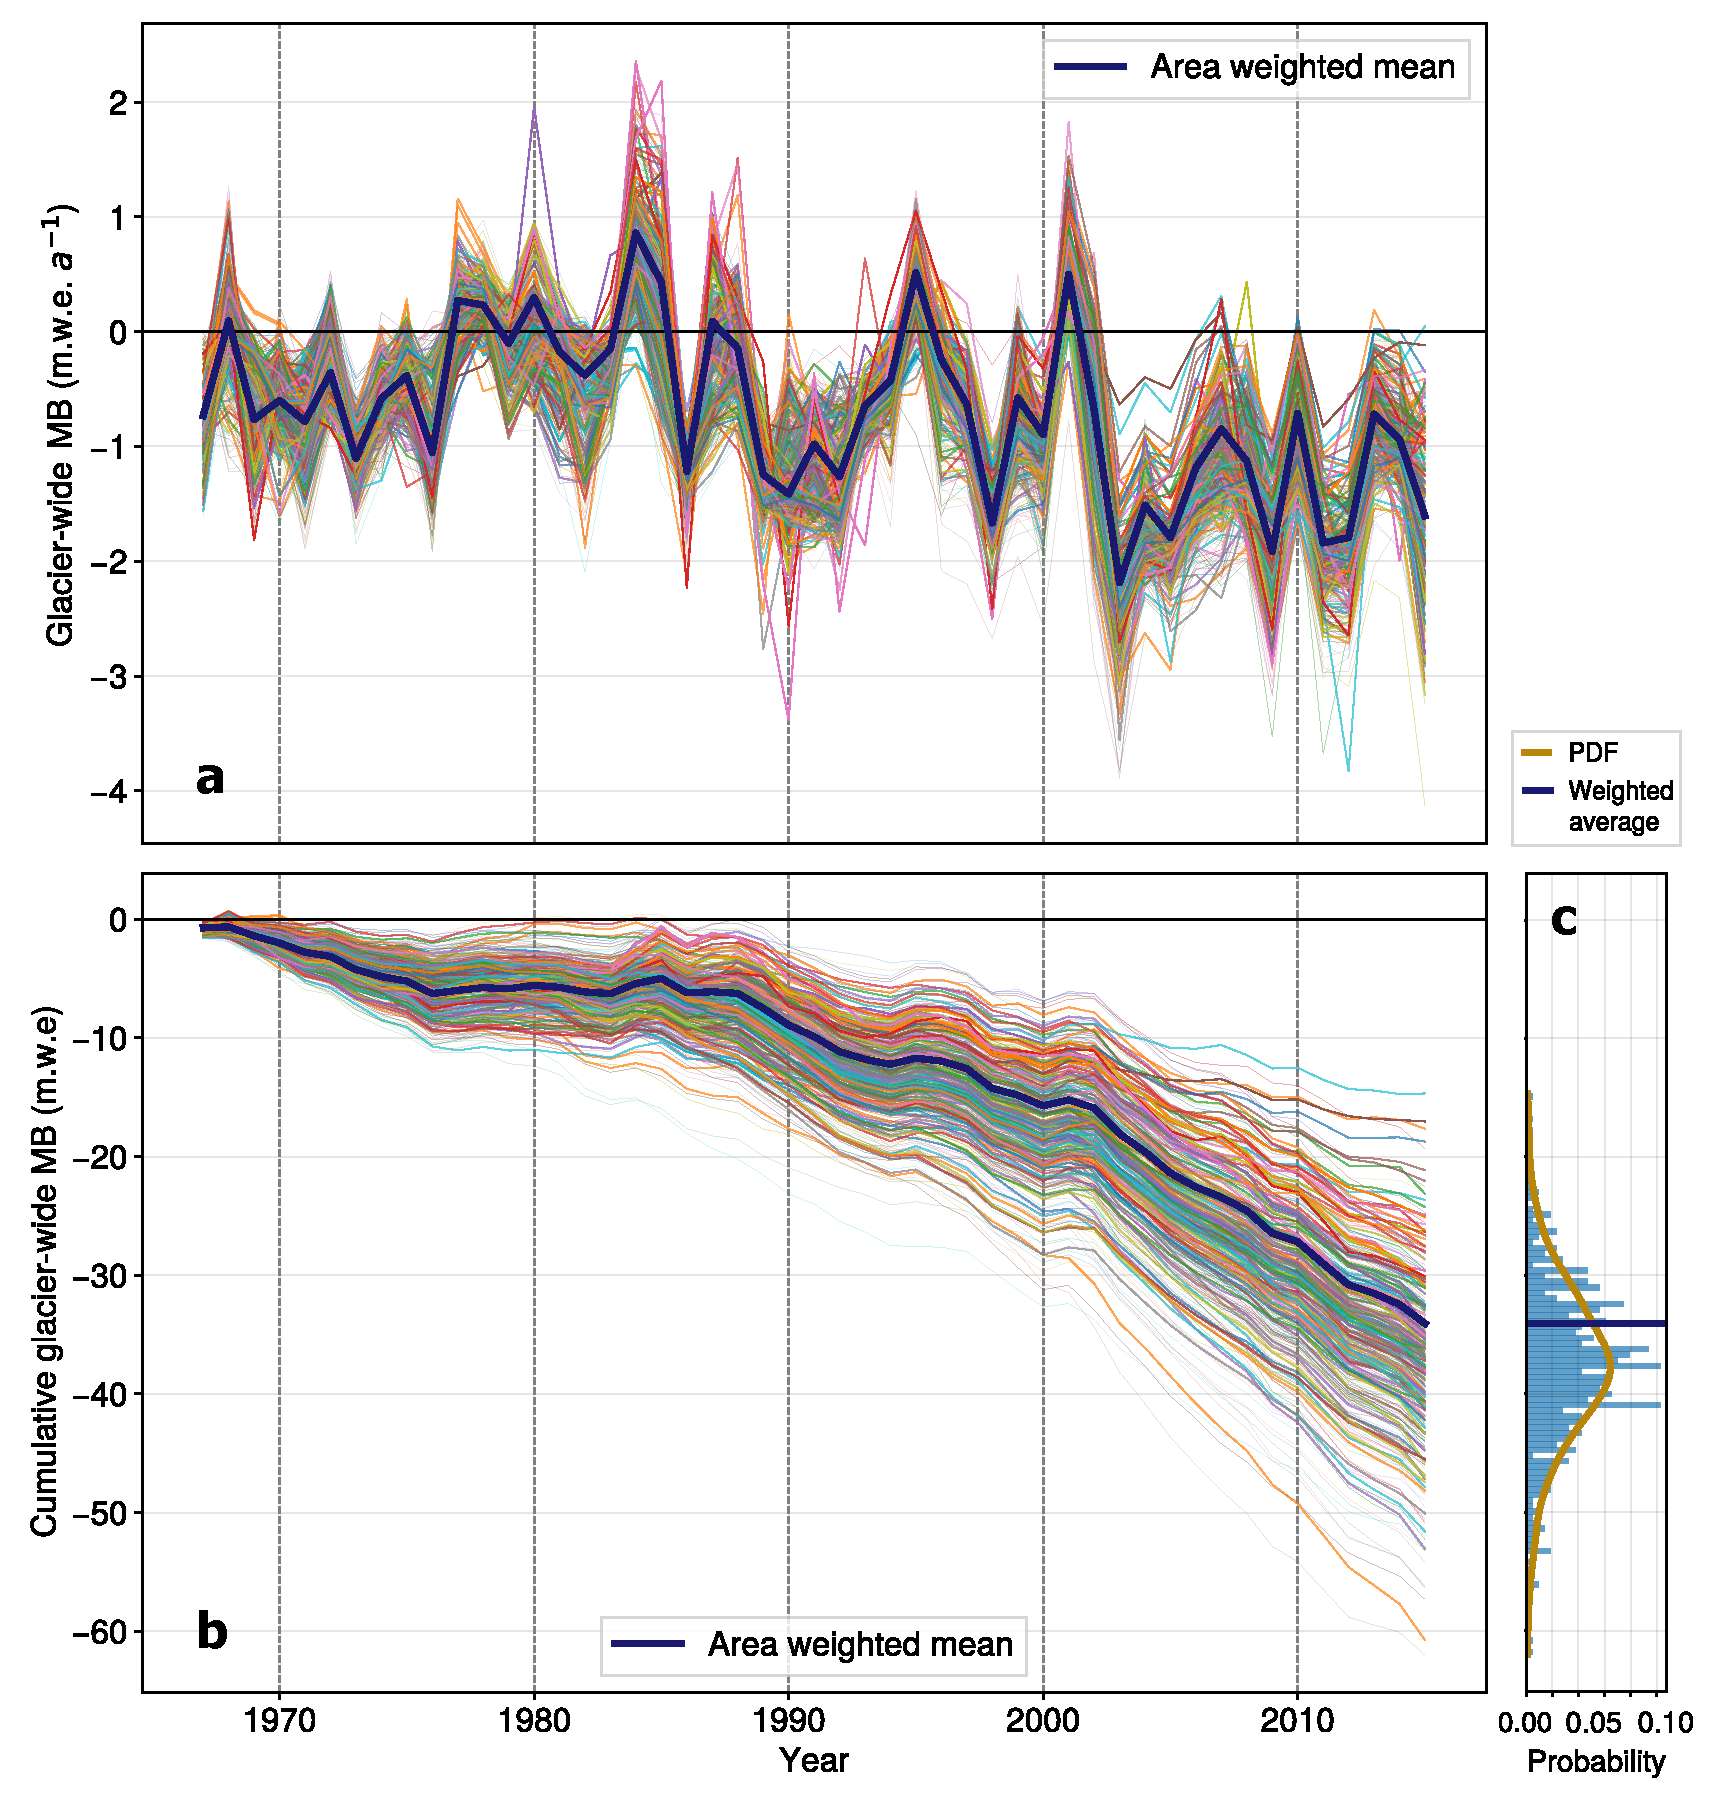
\includegraphics[width=10cm]{Figures/hydro/Figure_3.pdf}
\caption{Daily evolution of the glacierized surface area of Saint-Sorlin Glacier in J2K. Glacier retreat during the ablation season is well captured in the model, following the prescribed interpolated area evolution. The glacier area is only updated from October 2003 onwards, after the first year with available glacier ice thickness data.} 
\label{hydro:fig3}
\end{figure}

\subsection{Glacier mass balance}

This manual MB calibration enabled a correct representation of the MB of Saint-Sorlin Glacier, but the interannual variability is still not well captured, particularly for the 2005-2008 period (Fig. \ref{hydro:fig4}). An automatic calibration, testing a wide range of parameter configurations, would certainly yield a much better representation. The best results (annual RMSE = 2.20$^{9}$ L) were obtained by increasing precipitation on the glacier by 70\%, with a melt factor for ice of 4 mm/ºC, lower than the values of 5.2 mm/ºC found in the literature \citep{reveillet_which_2017}, and a melt factor for snow of 2.66 mm/ºC, also inferior than values indicated in the literature (4.2 mm/ºC). The melt factor for snow we calibrated ended up being the same as the one previously used for the whole catchment with outlet at Saint-Jean d'Arves. The resulting simulated winter MB estimates were less accurate (RMSE winter = 1.56$^{9}$ L) than summer estimates (RMSE summer = 1.11$^{9}$ L), which are very well captured by the model (Fig. \ref{hydro:fig4}b and \ref{hydro:fig4}c). 

\begin{figure}[h]
\centering
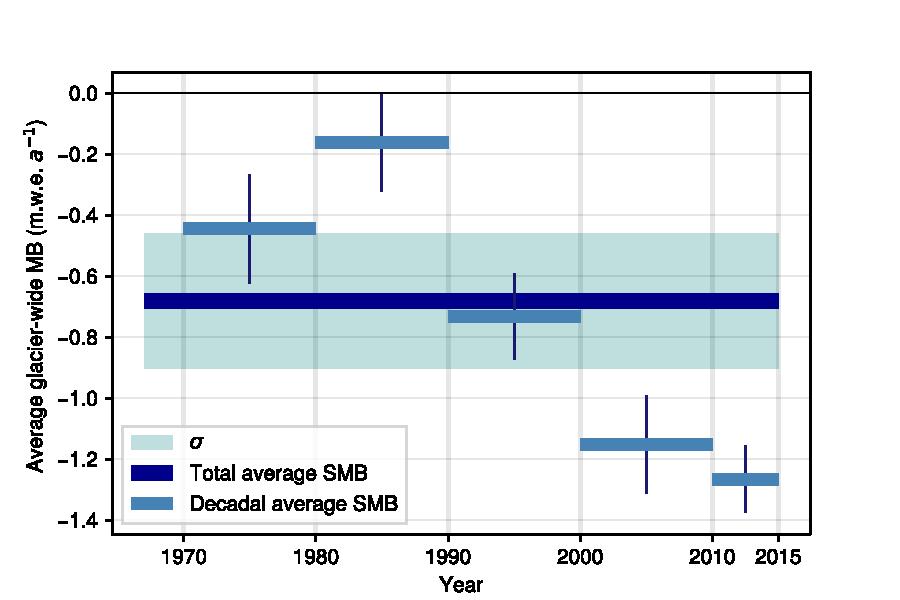
\includegraphics[width=15cm]{Figures/hydro/Figure_4.pdf}
\caption{Glacier-wide annual (a), seasonal winter (b) and summer (c) MB for Saint-Sorlin Glacier, with glaciological observations from the GLACIOCLIM observatory and simulated MB from J2K. Winter snowfall (d) and temperature (h), and summer snowfall (g) and temperature (i) are computed as an average of the four HRUs of the glacier. They are shown in order to give context on the meteorological conditions for those years.} 
\label{hydro:fig4}
\end{figure}

\subsection{Glacier runoff}

Runoff values in J2K are extracted at Saint-Jean d'Arves, where observations from the gauging station are available (Fig. \ref{hydro:fig1}). A comparison between the observed and the simulated daily discharges reveals a correct agreement between both (Fig. \ref{hydro:fig5}), displaying a Kling-Gupta Efficiency (KGE) of 0.69 and a Nash-Sutcliffe Efficiency (NSE) of 0.41. The addition of the glacier module improves the average monthly runoff distribution, allowing a better representation of the tail of late summer and early autumn glacier discharge contributions (Fig. \ref{hydro:fig5}). When looking specifically at the snow (March-June) and ice (July-October) melt seasons, the updated glacier module also manages to improve the performance of the simulated discharge, especially for the ice melt season (Table \ref{hydro:table1}). 

\begin{figure}[h]
\centering
\includegraphics[width=11cm]{Figures/hydro/Figure_5.pdf}
\caption{Average monthly runoff from the gauging station at Saint-Jean-d'Arves La Villette and from J2K simulations with and without the glacier.} 
\label{hydro:fig5}
\end{figure}

The total runoff contribution of the Saint-Sorlin Glacier is found to be quite important during the summer and autumn period, with peak monthly contributions ranging between 40-80\% and annual contributions between 17-35\%. By separating the net glacier contributions (only ice melt) from the total glacier contributions, we can observe how the ice melt contributions greatly vary between years depending on the late spring and summer snowpack characteristics (Fig. \ref{hydro:fig6}). The highest glacier contributions are found to have occured in the years 2003, with its famous summer heatwave, and the year 2009.

\begin{table}[h!]
\centering
\begin{tabular}{ | m{3cm} | m{3cm} | m{3.5cm}|} 
 \hline
   & \textbf{J2K with glacier} & \textbf{J2K without glacier} \\
 \hline \textbf{KGE}  & 0.69  & 0.66 \\
 \hline \textbf{KGE snow melt}  & 0.71  & 0.69 \\
 \hline \textbf{KGE ice mel}t  & 0.55  & 0.45 \\
 \hline \textbf{NSE}  & 0.41  & 0.36 \\
 \hline \textbf{NSE snow melt}  & 0.41  & 0.37 \\
 \hline \textbf{NSE ice melt}  & 0.11  & -0.15 \\
\hline
\end{tabular}
\caption{Performance of J2K discharge simulations at Saint-Jean d'Arves with and without the updated glacier module. The snow melt period is computed as the runoff between March-June and the ice melt period as the runoff between July-October.}
\label{hydro:table1}
\end{table}

\begin{figure}[h]
\centering
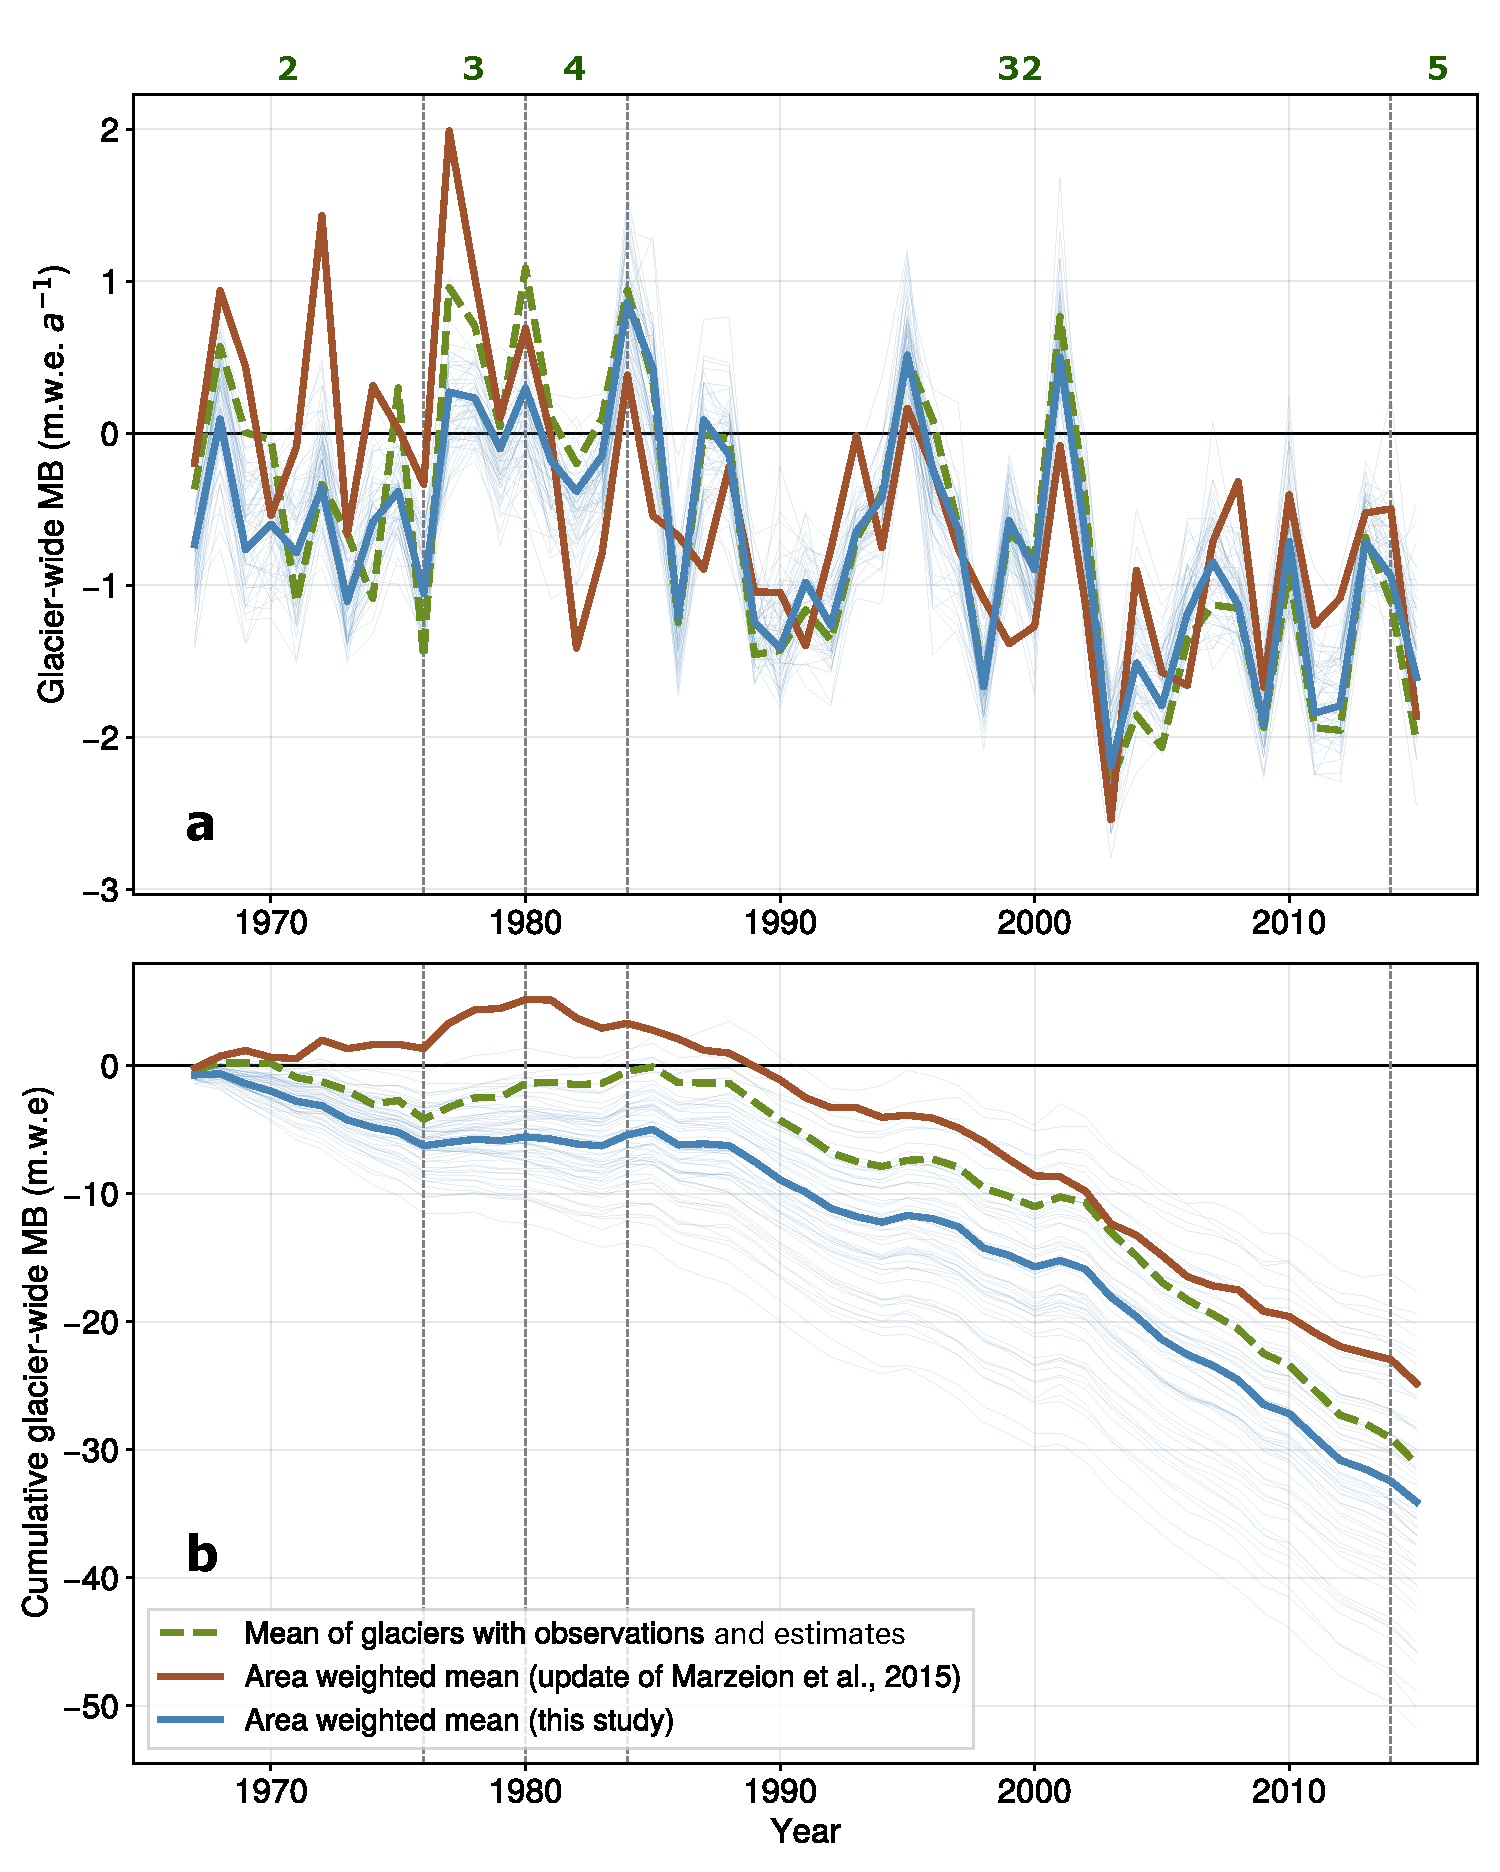
\includegraphics[width=11cm]{Figures/hydro/Figure_6.pdf}
\caption{(a) Monthly total and net (only ice melt) glacier contributions to the total catchment discharge, and (b) annual total and net glacier contributions.} 
\label{hydro:fig6}
\end{figure}

\section{Discussion and conclusions}

We introduced an updated glacier module for the J2K distributed process-based hydrological model, allowing a representation of glacier dynamics. This updated glacier module was applied to the Arvan glacierized catchment in the French Alps as a case study, in order to (a) demonstrate the capability of including glacier dynamics in the J2K model based on ALPGM outputs and (b) highlight the added value of the representation of glaciers within a hydrological model operating in high-altitude, partially glacierized alpine catchments. The addition of glacier dynamics can benefit hydrological models in their current representation of the hydrological regimes of glacierized catchments, but it is especially expected to be of great importance to future hydrological projections, when glacier shrinkage will drive significant changes at catchment scale \citep{hock_high_2019}. Physical realism of hydrological models has been long sought as an important asset to improve their performance and predictive power \citep{hrachowitz_decade_2013}, notably with an aim of ensuring the reliability of simulations in future projections \citep[e.g.][]{gao_prediction_2020}. Despite the small changes in glacier area in this case study (Fig. \ref{hydro:fig3}), we showed that the updated glacier module enabled an improved representation of both monthly runoff distribution (Fig. \ref{hydro:fig5}) and daily discharge rates, with an improved KGE and NSE (Table \ref{hydro:table1}). The most important differences were related to the glacier discharge contributions between late summer and autumn, when the net glacier runoff contributions are the highest. The discharge contributions from these months will also be the most severely affected by glacier retreat, indicating the progressive transition from a glacio-nival regime to a nival regime \citep{hock_high_2019}. The here presented developments are necessary to carry on realistic simulations of the Arvan and most high altitude partially glacierized catchments for the coming decades. 

We leveraged the seasonal GLACIOCLIM MB data to perform a stepwise calibration of the glacier specific parameters: the precipitation corrective factor (based on winter MB only) and the ice melt factor (based on summer MB only. As found in previous studies \citep{schaefli2011MassBalance}, this resulted in a realistic simulation of both MB components, while the agreement with the annual MB observations only led to some equifinality between these parameters and precluded the selection of a physically sound solution. For the present study we re-used a snow melt factor that had been adjusted through automatic calibration based on river discharge at the catchment outlet in previous simulations without the updated glacier module. A recalibration of this parameter could have been performed in the stepwise framework, based on river discharge during the snow melt period (March to late June). Nonetheless, we were obliged to shorten the calibration phase due to time constrains. For the vast majority of French Alpine glaciers no seasonal MB observations are available. In order to overcome this limitation, a potential strategy would be to use MB reconstructions from ALPGM produced during this PhD work \citep{bolibar_deep_2020-3}, in order to calibrate the parameters from the MB model \citep{stahlEA2008}, implying a revision of the calibration strategy for J2K. Following \citet{KonzSeibert2010}, we hypothesize that the ice melt factor could be calibrated based on late summer and early autumn discharge at the catchment outlet, a period when glacier contribution to the flow is essential, provided that the glacierized fraction of the catchment is not negligible. Indeed, these authors found that only three days of discharge measurements from the melt period can already help calibrate the parameters of a glacio-hydrological model. Then, the precipitation multiplication factor could be calibrated to ensure that the annual glacier-wide MB is respected. The possibilities and limitations of this strategy should be first evaluated on glaciers and catchments with seasonal MB estimates, such as the Arvan case study. 

Therefore, this implemented approach could be easily extended to all glaciers in the French Alps, as well as to glacierized catchments with multiple glaciers. J2K has already been deployed, adjusted and evaluated at the scale of the whole Rhone river basin which encompasses all glaciers from the French Alps \citep{braud_j2000-rhone_2017}. Similarly, ALPGM provides a regional glacier reconstruction and projection tool for the French Alps, so that the combination of both models enables glacio-hydrological simulations and projections at this scale. Every HRU in J2K has an ID which can be matched to any Randolph Glacier Inventory (RGI) ID, allowing a specific calibration of melt and precipitation factors for each individual glacier. In catchments with small glaciers located close together, these might end up sharing an HRU. For these cases, the optimization of the melt model would have to be shared among all the glaciers present in that HRU. Alternatively, the size of the HRU separation can be reduced, improving the spatial representation of the catchment. Nonetheless, this has an important computational cost. We believe this updated modelling framework has enough flexibility to enable an accurate calibration of different melt factors and precipitation lapse rates in mountainous regions. The modelling framework of J2K includes a large array of components representing different processes related to snow and ice. This level of detail, together with the code execution efficiency of Java allow a detailed representation of the many processes involved in the high-altitude water cycle at large geographical scales. 

We expect this updated glacier module to become a key component for J2K to correctly assess the impacts of future glacier retreat of glacierized catchments. For the case of the French Alps and the BERGER project, it will be applied at a regional scale in order to simulate the future hydrological changes of all glacierized catchments in the French Alps. Unlike the recent study by \citet{laurent_impact_2020} in the Mont-Blanc massif, the choice of a process-based, distributed hydrological model opens the way to diverse applications that require knowledge of the different runoff components, including glacier contributions in diverse, mostly ungauged, locations of the catchment. The future regional ALPGM-J2K simulation results will enable biologists to assess the potential impacts of climate change and glacier retreat on aquatic biodiversity. The expected decrease of late summer and autumn runoff, the increase in summer water temperature and changes in sediment loads will alter the habitat of many aquatic species, making it possible for new species to move in and increase competition with already vulnerable ones \citep{robinson_ecosystem_2014}. Moreover, since many studies have already used J2K in glacierized regions, particularly in the Himalayas \citep{gao_test_2012, nepal_understanding_2014, nepal_space-time_2020}, this updated glacier module can be easily reused by other experienced scientists. By contributing to an open-source hydrological model with such a broad international community, we increase the impact and transferability of this work, following the principles that have guided the preceding chapters. 

\section{Code availability}

The source code of the Python package \textit{Glaciers-to-J2K} is available in the following GitHub repository: https://github.com/JordiBolibar/Glaciers-to-J2K


